\documentclass[a4paper,12pt]{article}
\usepackage{authblk}
\usepackage{xcolor}
\usepackage{graphicx}
\usepackage[round]{natbib}

\begin{document}
\title{My first document}
\author[1]{F. Batsleer}
\affil[1]{Terec}
\date{12-03-2018}
\maketitle


%\clearpage

\tableofcontents
\clearpage
My first \LaTeX{} document! Yeay!\\
\section{Introduction}
This will be the intro
\subsection{First part of introduction}

\section{Typesetting}
\subsection{Exercise 2}
This is my {\huge introduction}, I want to tell you something {\tiny really}, {\small really}, really, {\color{orange} \Large really}  \underline{incredible}.\\
My article is \textsc{amazing}.\\
It's \textbf{great}, just great.\\
\textit{Believe me}, we're going to make the \textsc{\color{green} TerecEonLimno} great again!\\

\subsection{Exercise 3}
\begin{enumerate}
	\item Department Biology
	\begin{itemize}
		\item Terec
		\begin{itemize}
			\item Dries Bonte
			\item Luc Lens
		\end{itemize}
		\item Eon
		\begin{itemize}
			\item[$\ast$] Matthew Shawkey
		\end{itemize}
		\item Limno
		\begin{itemize}
			\item[$\ast$] Dirk Verschuren
		\end{itemize}
	\end{itemize}
	\item Department Forest and Water Management
	\begin{itemize}
		\item ForNaLab
		\begin{itemize}
			\item[$\rightarrow$] Kris Verheyen
			\item[$\rightarrow$] Lander Baeten
			\item[$\rightarrow$] Pieter De Frenne
			\item[$\rightarrow$] Jan Mertens
		\end{itemize}
	\end{itemize}
\end{enumerate}

\section{Maths}
\subsection{Exercise 4}
...equation \ref{crazy-formula} was used to calculate this metric.
\begin{equation}\label{crazy-formula}
K = \sum_{i=0}^{i=n}\frac{\sqrt{\alpha}}{\delta_{ij}}
\end{equation}


\section{Tables \& Figures}
\subsection{Exercise 5}
\begin{table}[h]
	\begin{tabular}{l|c c c}
		 & & Year & \\
		 \cline{2-4}
		City & 2006 & 2007 & 2008\\
		\hline
		London & 45.000 & 46.000 & 51.000\\
		Berlin & 35.000 & 33.000 & 30.000\\
		Paris & 50.000 & 51.000 & 52.000\\
	\end{tabular}	
\end{table}

\subsection{Exercise 6}
\begin{figure}[ht]
	\centering
	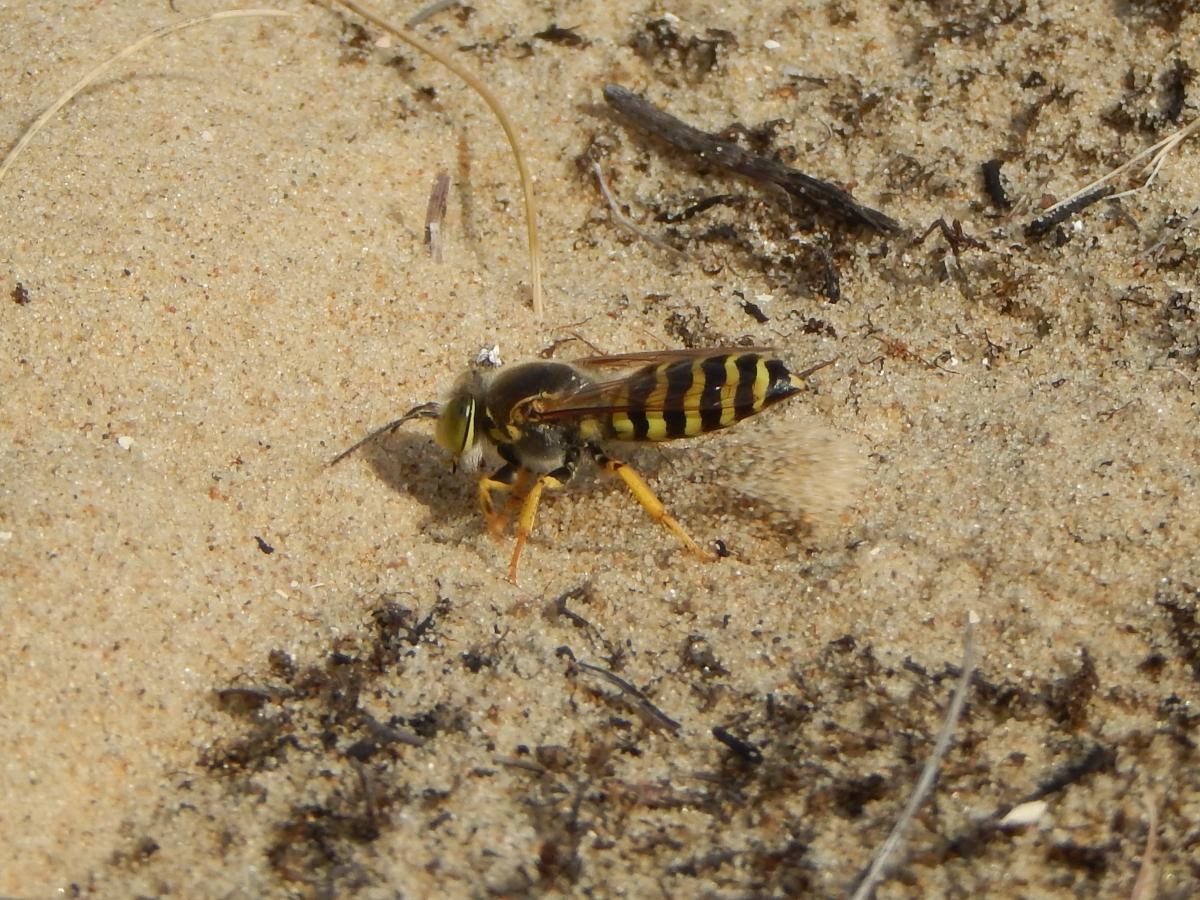
\includegraphics[height=0.5\textwidth]{DiggerWasp.jpg}
	\caption{What an amazing digger wasp!}\label{fig:diggerwasp}
\end{figure}

\section{References}
\subsection{Exercise 7}
\citeauthor{Tengo1996} say that a digger wasp needs $\pm$ 12 days to finish a nest cycle, provisioning its single larva with flies \citep{Nielsen1945}.

\section{Bibliography}
\bibliographystyle{ecol_let}

\bibliography{ExampleExport}

\end{document}